\documentclass[12pt,a4paper]{article}
%\usepackage{ctex}
\usepackage{amsmath,amscd,amsbsy,amssymb,latexsym,url,bm,amsthm}
\usepackage{epsfig,graphicx,subfigure}
\usepackage{enumitem,balance}
\usepackage{wrapfig}
\usepackage{mathrsfs,euscript}
\usepackage[usenames]{xcolor}
\usepackage{hyperref}
\usepackage[vlined,ruled,linesnumbered]{algorithm2e}
\hypersetup{colorlinks=true,linkcolor=black}
\usepackage{fancyhdr}
\usepackage{longtable}
\usepackage{array}
\usepackage{booktabs}
\usepackage{amsmath}
%\usepackage{algorithm}
%\newtheorem{theorem}{Theorem}
%\newtheorem{lemma}[theorem]{Lemma}
%\newtheorem{proposition}[theorem]{Proposition}
%\newtheorem{corollary}[theorem]{Corollary}
%\newtheorem{exercise}{Exercise}
%\newtheorem*{solution}{Solution}
%\newtheorem{definition}{Definition}
%\theoremstyle{definition}

\renewcommand{\thefootnote}{\fnsymbol{footnote}}

\newcommand{\postscript}[2]
 {\setlength{\epsfxsize}{#2\hsize}
  \centerline{\epsfbox{#1}}}
  

\renewcommand{\baselinestretch}{1.0}

\setlength{\oddsidemargin}{-0.365in}
\setlength{\evensidemargin}{-0.365in}
\setlength{\topmargin}{-0.3in}
\setlength{\headheight}{0in}
\setlength{\headsep}{0in}
\setlength{\textheight}{10.1in}
\setlength{\textwidth}{7in}

\pagestyle{fancy}{
\lhead{}
\chead{report of project2}
\fancyhead[RO]{Team 25}
\cfoot{\thepage}
\renewcommand{\headrulewidth}{\textwidth}
\vspace{6mm}
}
\title{Logistic service scheduling}
\author{Name: Yiting Chen  ID: 517021910169 Email: ytchen981@163.com 
 }
\date{\today}

\begin{document}
\maketitle
\begin{abstract}
Reasonable scheduling of logistics service supply chain is essential. To minimize the total cost of the service, minimize the difference between the total service time and the customers; requirement and maximize the satisfaction, we established two scheduling models with fixed customer order decoupling point(CODP). One model ignores the relationship between the time window of supplier operation and the customer requirement and focus on the cost and satisfaction, while the other one considering the relationship. We convert the multiple-objective programming model into a LP problem and solve it with Cplex.
\end{abstract}
\renewcommand{\contentsname}{catalog}
\tableofcontents
\newpage
\ \\
\section{Introduction}
Nowadays logistics enterprises provide mass customization logistics services(MCLS) which allows customer to  request customization service or mass service. To provide better service, the logistics service integrator need to reduce the cost, satisfy the customers' time requirement and keep functional logistic service providers satisfied. Our report focus on the schedule model in the two-echelon logistic service supply chain. This paper is organized as follows. In \textbf{section 2}, we introduce our schedule model regarding the problem. In \textbf{section 3}, we analyze the problem and the algorithm to solve the problem. In \textbf{section 4}, we analyze the time complexity of the algorithm and evaluate the performance of our model with the given data. The reference section and acknowledge section are given respectively at the end. 

\section{Model building}
\subsection{Problem describing}    
Assume there is a two-echelon logistics service supply chain(LSSC) with one logistics service integrator(LSI) and many functional logistic service providers(FLSP). The LSI may receive many orders from customers at a time. Each order consists of multiple service processes, which can be divided into two types, the customized service process and the mass service process. The service process of customers is conducted either being integrated into the mass service process or being operated independently as customized service. The LSI analyses the demand from customer and inquires the FLSPs of each service process about the time window for completing the service process.Then the LSI needs to schedule the orders and determine which process are conducted in mass mode and which are in customized mode.For example, there are three customers:
\begin{figure}[h]
\centering
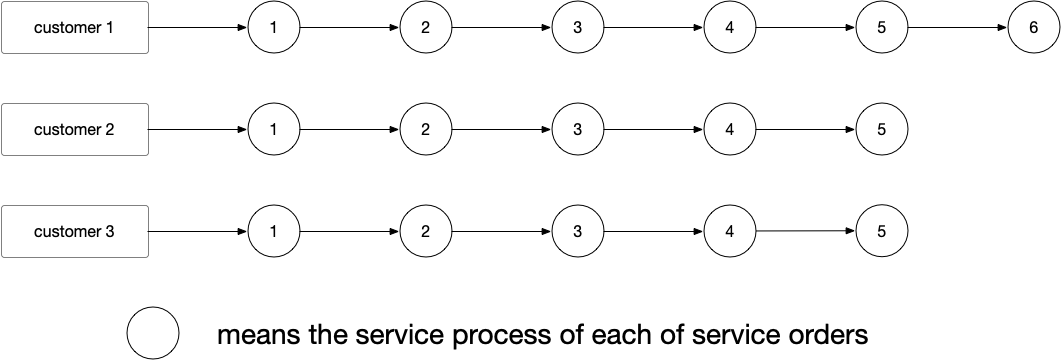
\includegraphics[width=0.8\textwidth]{figures/fig1.png}
\caption{Example of customer requeset}
\end{figure}
Then the LSI would determine the CODP and execute some of the processes in mass service and others in customized service.
\begin{figure}[htbp]
\centering
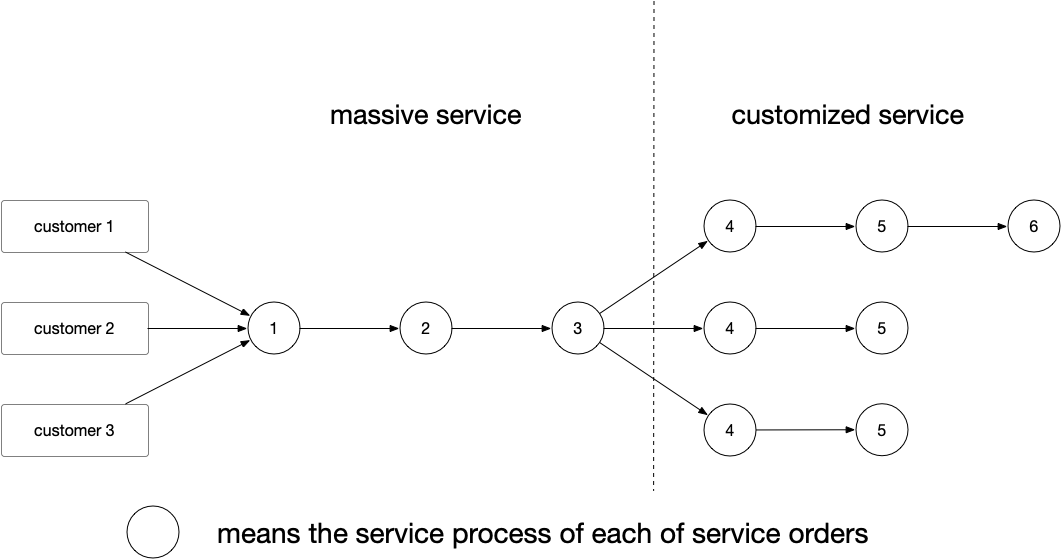
\includegraphics[width=0.8\textwidth]{figures/fig2.png}
\caption{Demonstration of the actual service}
\end{figure}
Our goal is schedule the processes and met the goals.
\newpage
\subsection{Notation}
The notation of the model are as follows:
\begin{longtable}[b]{p{3cm}p{12cm}}
			%\specialrule{0.05em}{3pt}{3pt}
\hline
Notation & Description\\
			\specialrule{0.05em}{3pt}{3pt}
$T_i^{exp}$ & The expect time for FLSP to complete $i$th process in offering mass service\\
			\specialrule{0.05em}{3pt}{3pt}
$T_i$ & The actual time FLSP takes to complete $i$th process in offering mass service\\
			\specialrule{0.05em}{3pt}{3pt}
$T_i^{ext}$ & The time LSI scheduled for $i$th process in mass service\\
\specialrule{0.05em}{3pt}{3pt}
$T_{ij}^{exp}$ & The expect time for FLSP to complete $i$th process in customized mode for customer $j$\\
\specialrule{0.05em}{3pt}{3pt}
$T_{ij}$ & The actual time FLSP takes to complete $i$th process in customized mode for customer $j$\\
\specialrule{0.05em}{3pt}{3pt}
$T_{ij}^{ext}$ & The time LSI scheduled for customer $j$ in $i$th process\\ 
\specialrule{0.05em}{3pt}{3pt}
$T_j^{exp}$ & The custmoer $j$'s expected completion time\\
\specialrule{0.05em}{3pt}{3pt}
$T_{i+1}^+$ & In mass processes, the upper limit of the time delay incurred in the (i − 1)th service process which could be endured by the ith service process. It is determined by the rigid requirement caused by upstream and downstream operations of LSSC.\\
\specialrule{0.05em}{3pt}{3pt}
$T_{i+1}^-$ & In mass processes, the upper limit of the time ahead of schedule incurred in the (i − 1)th service process which could be endured by the ith service process, which is determined by the rigid requirement caused by upstream and downstream operations of LSSC.\\
\specialrule{0.05em}{3pt}{3pt}
$T_{(i+1)j}^+$ & In customized processes, for the jth customer order, the upper limit of the time delay incurred in the (i − 1)th service process which could be endured by the ith service process, which is determined by the rigid requirement caused by upstream and downstream operations of LSSC.\\
\specialrule{0.05em}{3pt}{3pt}
$T_{(i+1)j}^-$ & In customized processes, for the jth customer order, the upper limit of the time ahead of schedule incurred in the (i − 1)th service process which could be endured by the ith service process, which is determined by the rigid requirement caused by upstream and downstream operations of LSSC.\\
\specialrule{0.05em}{3pt}{3pt}
$C_i$ & The normal cost per unit time of $i$th process in offering mass service\\
\specialrule{0.05em}{3pt}{3pt}
$C_i^{ext}$ & The extra cost per unit time of $i$th process in offering mass service\\
\specialrule{0.05em}{3pt}{3pt}
$C_{ij}$ & The normal cost per unit time of $i$th process in offering customized service for customer $j$\\
\specialrule{0.05em}{3pt}{3pt}
$C_{ij}^{ext}$ & The extra cost per unit time of $i$th process in offering customized service for customer $j$\\
\specialrule{0.05em}{3pt}{3pt}
$P_{i}$ & The penalty per unit time of $i$th process in mass service if order is finished ahead of the expected time \\
\specialrule{0.05em}{3pt}{3pt}
$P_{ij}$ & The penalty per unit time of $i$th process in customized service for customer $j$ if order is finished ahead of the expected time\\
\specialrule{0.05em}{3pt}{3pt}
$U_i$ & The lower limit of the satisfaction degree of the $i$th mass process. \\
\specialrule{0.05em}{3pt}{3pt}
$U_{ij}$ & The lower limit of the satisfaction degree of the ith customized process of the jth customer order.\\
\specialrule{0.05em}{3pt}{3pt}
$Z_1$ & The total cost\\
\specialrule{0.05em}{3pt}{3pt}
$Z_2$ & The satisfaction\\
\specialrule{0.05em}{3pt}{3pt}
$Z_3$ & The closeness degree of the actual order completion time and its customer requirement.\\
\specialrule{0.05em}{3pt}{3pt}
$k$ & Before $k$th process the service is mass and after it will be customized\\
\specialrule{0.05em}{3pt}{3pt}
$Y$ & The total number of orders\\
\specialrule{0.05em}{3pt}{3pt}
$Y_j$ & The number of orders from $j$th customer\\
\specialrule{0.05em}{3pt}{3pt}
$c$ & The cost coefficient\\
\specialrule{0.05em}{3pt}{3pt}
$\beta$ & The requirement coefficient\\ 
\specialrule{0.05em}{3pt}{3pt}
$I_j$ & The number of processes in $j$th customer's order\\
\specialrule{0.05em}{3pt}{3pt}
$J_0$ & The number of customers\\
			\hline
\caption{notation of the model}
\end{longtable}
\subsection{Assumption}
According to the description we have following assumptions:
\begin{enumerate}
\item Each scheduling task aims at only one set of customer orders and no new orders are added
\item In terms of time scheduling, additional service costs are incurred.
\item The normal service time refers to the usual time needed in completing a task using FLSP capability. When the work is done in the expect time, the satisfaction of the FLSPs is the highest.
\item We assume that logistics service capacities in each process are adequate and thus there is not any capacities constraint.
\end{enumerate}

\subsection{Model Building}
\subsubsection{The model without the Relationship between Time Windows of Supplier Operation and Customer Requirement}
In the problem, the object is to reduce the cost $Z_1$ and increase the satisfaction $Z_2$.
We calculate the cost $Z_1$ as follows:
\begin{equation}
	Z_1=f_1+f_2+f_3
\end{equation}
where
\begin{equation}
	f_1 =\sum_{i=1}^{i=k-1}(T_iC_i+|T_i^{ext}|C_i^{ext})\times Y\\
\end{equation}
\begin{equation}
	f_2 =\sum_{i=k}^{I_j}\sum_{j=1}^{J_0}(T_{ij}C_{ij}+|T_{ij}^{ext}|C_{ij}^{ext})\times Y_j\\
\end{equation}
\begin{equation}
	f_3=\sum_{i=1}^{i=k-1}|(T_i^{exp}-T_i-T_i^{ext})|P_i\times Y+\sum_{i=k}^{I_j}\sum_{j=1}^{J_0}|(T_{ij}^{exp}-T_{ij}-T_{ij}^{ext})|P_{ij}\times Y_j\\
\end{equation}
$f_1$ is the cost of mass service and $f_2$ is the cost of customized service. $f_3$ is the penalty.\\
We define the satisfaction $Z_2$ via the relationship between the expected time and the actual time and the relationship between the cost of normal service and the total cost\cite{Liu}:
\begin{equation}
\begin{split}
	Z_2=(\sum_{i=1}^{i=k-1}(1-|\frac{T_i^{exp}-T_i}{T_i^{exp}}|)(\frac{T_iC_i}{T_iC_i+T_i^{ext}C_i^{ext}})+\sum_{i=k}^{I_j}\sum_{j=1}^{J_0}(1-|\frac{T_{ij}^{exp}-T_{ij}}{T_{ij}^{exp}}|)(\frac{T_{ij}C_{ij}}{T_{ij}C_{ij}+T_{ij}^{ext}C_{ij}^{ext}}))\\
	\times(k-1+\sum_{j=1}^{J_0}(I_j-(k-1)))^{-1}
\end{split}
\end{equation} 
As for restraints:
\begin{equation}
	T_{i+1}^-\leq T_i^{exp}-T_i-T_i^{ext}\leq T_{i+1}^+ \quad ,i\leq k-1\\
\end{equation}
\begin{equation}
	T_{(i+1)j}^-\leq T_{ij}^{exp}-T_{ij}-T_{ij}^{ext}\leq T_{(i+1)j}^+ \quad, i>k\\
\end{equation}
\begin{equation}
	(1-|\frac{T_i^{exp}-T_i}{T_i^{exp}}|)(\frac{T_iC_i}{T_iC_i+T_i^{ext}C_i^{ext}})\geq U_i\\
\end{equation}
\begin{equation}
	(1-|\frac{T_{ij}^{exp}-T_{ij}}{T_{ij}^{exp}}|)(\frac{T_{ij}C_{ij}}{T_{ij}C_{ij}+T_{ij}^{ext}C_{ij}^{ext}})\geq U_{ij}\\
\end{equation}
Because $Z_2\in \{0,1\}$.Simplify the multiobjective programming model, We get:
\begin{alignat}{2}
\min \quad & K_1Z_1+K_2Z_1^{min}(1-Z_2)\\
\mbox{s.t.}\quad
& T_{i+1}^-\leq T_i^{exp}-T_i-T_i^{ext}\leq T_{i+1}^+ \quad ,i\leq k-1\\
& T_{(i+1)j}^-\leq T_{ij}^{exp}-T_{ij}-T_{ij}^{ext}\leq T_{(i+1)j}^+ \quad, i\geq k\\
& (1-|\frac{T_i^{exp}-T_i}{T_i^{exp}}|)(\frac{T_iC_i}{T_iC_i+T_i^{ext}C_i^{ext}})\geq U_i\\
& (1-|\frac{T_{ij}^{exp}-T_{ij}}{T_{ij}^{exp}}|)(\frac{T_{ij}C_{ij}}{T_{ij}C_{ij}+T_{ij}^{ext}C_{ij}^{ext}})\geq U_{ij}\\
\end{alignat}
$K_1$ and $K_2$ represents the weight of $Z_1$ and $Z_2$.
\subsubsection{The model with the Relationship between Time Windows of Supplier Operation and Customer Requirement}
Considering the relationship between time windows of supplier operation and customer requirement, we introduce a new variable $Z_3$ to describe the closeness of the actual order completion time and its customer requirement.
\begin{equation}
	Z_3=\sum_{j=1}^{J_0}|\frac{T_j^{exp}-T_j}{T_j^{exp}}|\frac{1}{J_0}
\end{equation} 
where
\begin{equation}
	T_j=\sum_{i=1}^{I_j}(T_i+T_i^{ext}+T_{ij}+T_{ij}^{ext})
\end{equation}
$T_j$ is the actual time to complete customer$j$'s order.\\
Hence, there are three objects. To simplify the multiobjective programming model, we restrain $Z_1$ to 
\begin{equation}
 Z_1\leq Z_1^{min}\times(1+c)
\end{equation} 
where $c$ is the cost coefficient and 
\begin{equation}
Z_1^{min}= \sum_{i=1}^{i=k-1}T_iC_i\times Y+\sum_{i=k}^{I_j}\sum_{j=1}^{J_0}(T_{ij}C_{ij}\times Y_j
\end{equation}
Considering the requirement of the customer we also add a constraint of the time required by customers: $T_j\leq T_j^{exp}(1+\beta)$. Then we got:
\begin{alignat}{2}
\min \quad & K_3Z_3+K_2(1-Z_2)\\
\mbox{s.t.}\quad
& T_j\leq T_j^{exp}(1+\beta)\\
& T_{i+1}^-\leq T_i^{exp}-T_i-T_i^{ext}\leq T_{i+1}^+ \quad ,i\leq k-1\\
& T_{(i+1)j}^-\leq T_{ij}^{exp}-T_{ij}-T_{ij}^{ext}\leq T_{(i+1)j}^+ \quad, i\geq k\\
& (1-|\frac{T_i^{exp}-T_i}{T_i^{exp}}|)(\frac{T_iC_i}{T_iC_i+T_i^{ext}C_i^{ext}})\geq U_i\\
& (1-|\frac{T_{ij}^{exp}-T_{ij}}{T_{ij}^{exp}}|)(\frac{T_{ij}C_{ij}}{T_{ij}C_{ij}+T_{ij}^{ext}C_{ij}^{ext}})\geq U_{ij}\\
& Z_1\leq Z_{1min}
\end{alignat}
convert it into LP:
\begin{alignat}{2}
\min \quad & K_3Z_3+K_2(1-Z_2)\\
\mbox{s.t.}\quad
& T_j\leq T_j^{exp}(1+\beta)\\
& T_{i+1}^-\leq T_i^{exp}-T_i-T_i^{ext}\leq T_{i+1}^+ \quad ,i\leq k-1\\
& T_{(i+1)j}^-\leq T_{ij}^{exp}-T_{ij}-T_{ij}^{ext}\leq T_{(i+1)j}^+ \quad, i\geq k\\
& (1-|\frac{T_i^{exp}-T_i}{T_i^{exp}}|)^{-1}(1+\frac{T_i^{ext}C_i^{ext}}{T_iC_i})\leq U_i^{-1}\\
& (1-|\frac{T_{ij}^{exp}-T_{ij}}{T_{ij}^{exp}}|)^{-1}(\frac{T_{ij}^{ext}C_{ij}^{ext}}{T_{ij}C_{ij}})\leq U_{ij}^{-1}\\
& Z_1\leq Z_{1min}
\end{alignat}
$K_2$ and $K_3$ represents the weight of $Z_2$ and $Z_3$
\section{Problem Analysis and Algorithm Design}
Our defined problem is a multiple-objective programming problem. We simplify the problem with linear weight method and get the synthesized objective function. Our single-objective model could be converted into LP. Hence the defined problem should be in $P$ and we could use various algorithms to solve the problem. Using Ellipsoid Method the time complexity would be $O(n^6L^2)$ where $n$ is the dimension of variables and $L$ is the length of input. If we solve the problem using Interior-Point Method the time complexity would be $O(n^{3.5}L^2)$.\\
For example, Barrier Method\cite{Convex}:\\
\begin{algorithm}[H]
\caption{Barrier Method}
 given strictly feasible\\
 \While{True}{
	Centering step. Compute by minimizing, subject to, starting at.\\
	Update.\\
	Stopping criterion. quit if.\\
	increase.\\
	}
\end{algorithm}
In this project we use Cplex to solve the LP problem.
\newpage
\section{Theoretical Analysis and Performance Evaluation}
\subsection{Theoretical Analysis}
The time complexity is determined by the method we use to solve the LP problem. If we use simplex method, the time complexity is $O(2^n)$. If we use Ellipsoid Method the time complexity would be $O(n^6L^2)$. If we use Interior-Point Method, the time complexity would be $O(n^{3.5}L^2)$. We use Cplex to solve the LP problem.
\subsection{Performance Evaluation}
\subsubsection{Evaluation of the model without the Relationship between Time Windows of Supplier Operation and Customer Requirement}
For service time distribution, we generate the actual service time via a random function. The data we use are listed as follows:\\

The result is showed in the figures:\\

\subsubsection{Evaluation of the model with the Relationship between Time Windows of Supplier Operation and Customer Requirement}
In this model we have two coefficients $c$ and $\beta$.

\section*{Acknowledgement}
\begin{thebibliography}{1}
\bibitem{Liu}  Liu WH, Yang Y, Li X, Xu HT, Xie D. A time scheduling model of logistics service supply chain with mass customized logistics service. Discrete Dynamics in Nature and Society. 2012;2012:18 pages.482978
\bibitem{Convex} Stephen Boyd,Lieven Vandenberghe. Convex Optimization [M]
\end{thebibliography}
\
\end{document}